%%%%%%%%%%%%%%%%%%%%%%%%%%%%%%%%%%%%%%%%%%%%%%%%%%%%%%%%%%%%%%%%%%% 
%% Desarrollo -  Modelado en punto flotante
%%%%%%%%%%%%%%%%%%%%%%%%%%%%%%%%%%%%%%%%%%%%%%%%%%%%%%%%%%%%%%%%%%%
\subsection{Modelo en punto flotante}
\begin{frame}
  \frametitle{\textbf{Tabla de Contenidos}}
  \begin{center}
    {\vspace{-1.5cm}\Large \textbf{Sección \thesection: \secname }\vspace{0.5cm}}
    \begin{beamercolorbox}[
      sep=8pt,center]{part title}
      \usebeamerfont{part title}
      \textbf{\subsecname}
    \end{beamercolorbox}
  \end{center}
\end{frame}

\begin{frame}
  \frametitle{\textbf{Esquema de simulación}}
\framesubtitle{\secname : \subsecname}
    % \vspace{-0.3cm}

  \begin{figure}[!t] \centering
    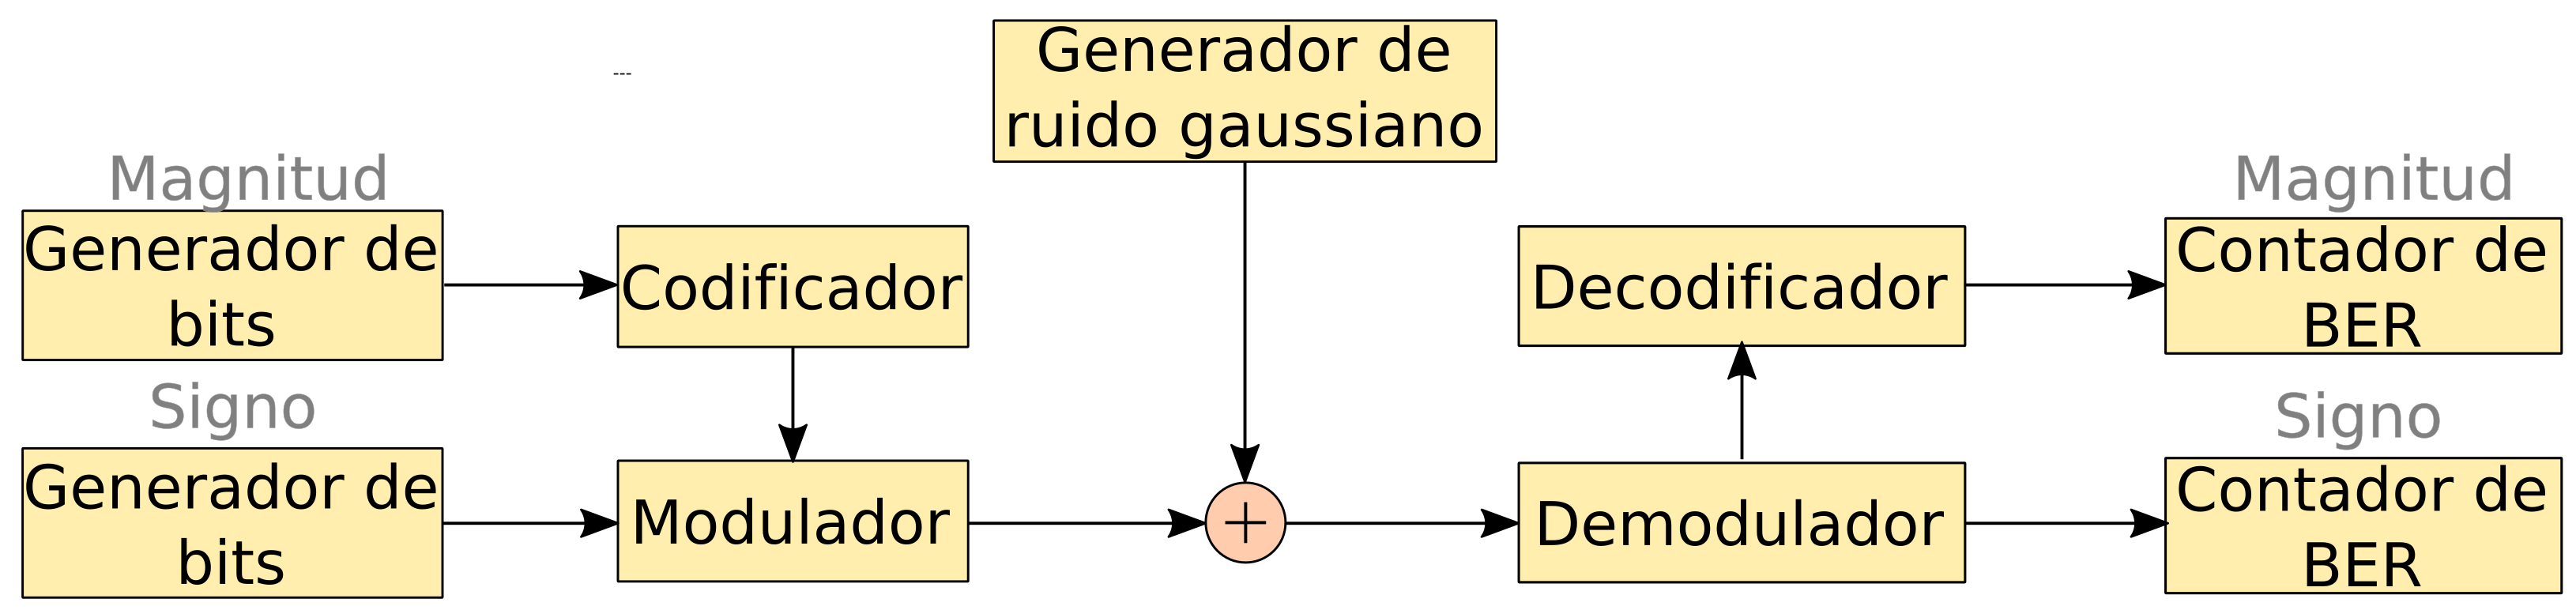
\includegraphics[width=0.85\paperwidth]{Diagramas/proyect_alto_nivel.png}%
  \end{figure}
  
  \vspace{-0.5cm}
  \noindent\rule{8cm}{0.4pt}\centering
  \vspace{-0.3cm}

  \begin{columns}
    \begin{column}{0.48\linewidth}  
        \begin{figure}
        \centering
        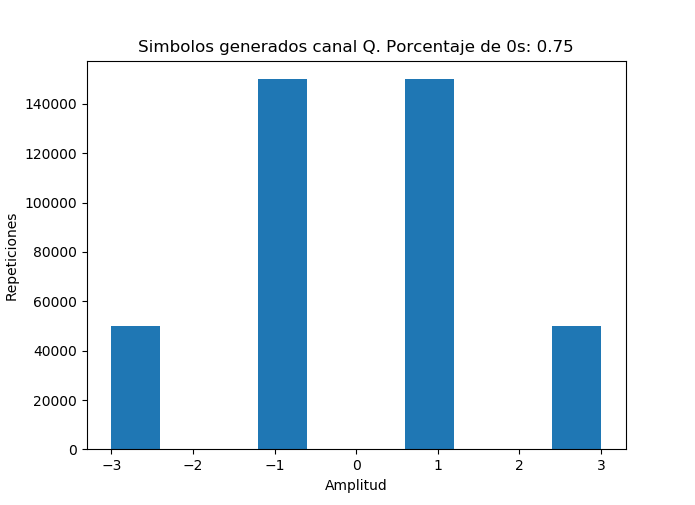
\includegraphics[width=\textwidth]{Graficos/coded_symbols_6.png}
        \end{figure}
    \end{column}
    \begin{column}{0.408\linewidth}
        \vspace{0.15cm}
        \begin{figure}
            \centering
            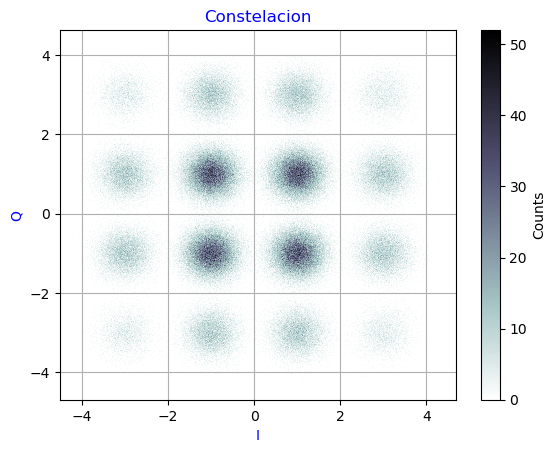
\includegraphics[width=\textwidth]{Graficos/Constellation_025.png}
        \end{figure}
    \end{column}
\end{columns}
  
\end{frame}

% \begin{frame}
%   \frametitle{\textbf{Resultados obtenidos}}
\framesubtitle{\secname : \subsecname}
% \begin{columns}
%     \begin{column}{0.48\paperwidth}  
%     \begin{figure}
%         \centering
%         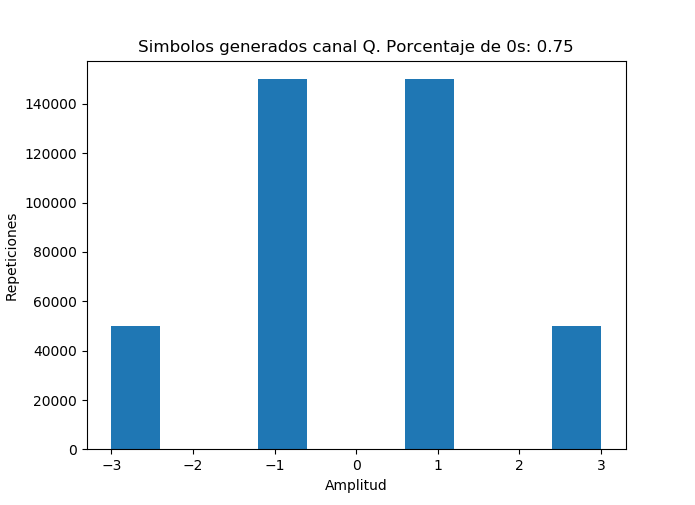
\includegraphics[width=\textwidth]{Graficos/coded_symbols_6.png}
%         \caption{Símbolos codificados, $P_{(x=0)}=0.75$}
%         %\label{fig:my_label}
%     \end{figure}
%     \end{column}

%     \begin{column}{0.48\paperwidth}
%     \begin{figure}
%         \centering
%         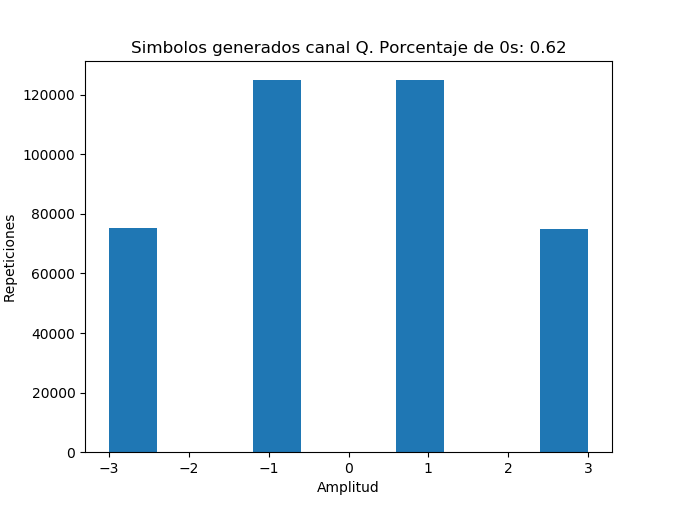
\includegraphics[width=\textwidth]{Graficos/coded_symbols_5.png}
%         \caption{Símbolos codificados, $P_{(x=0)}=0.62$}
%         % \label{fig:my_label}
%     \end{figure}
%     \end{column}
            
% \end{columns}
% \end{frame}

% \begin{frame}
%   \frametitle{\textbf{Resultados obtenidos}}
% \framesubtitle{\secname : \subsecname}
% %   Símbolos codificados, $P_{(x=0)}=0.75$
% %     \vspace{-0.3cm}

% \begin{columns}
%     \begin{column}{0.48\linewidth}  
%     \begin{figure}
%         \centering
%  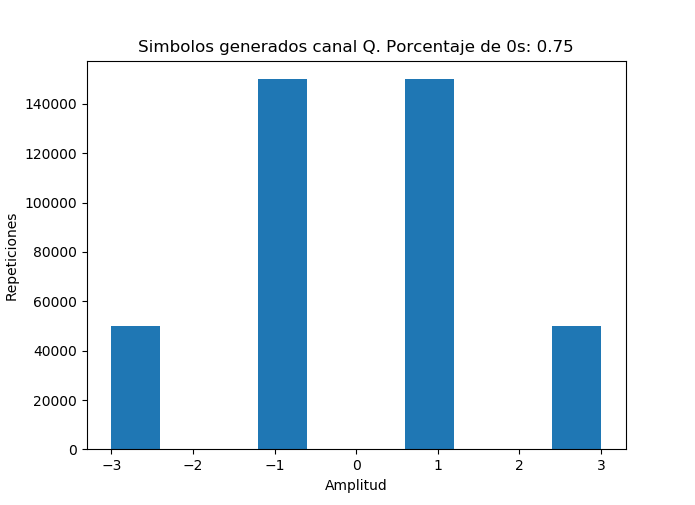
\includegraphics[width=\textwidth]{Graficos/coded_symbols_6.png}
%     \end{figure}
%     \end{column}

%     \begin{column}{0.43\linewidth}
%     \begin{figure}
%         \centering
%         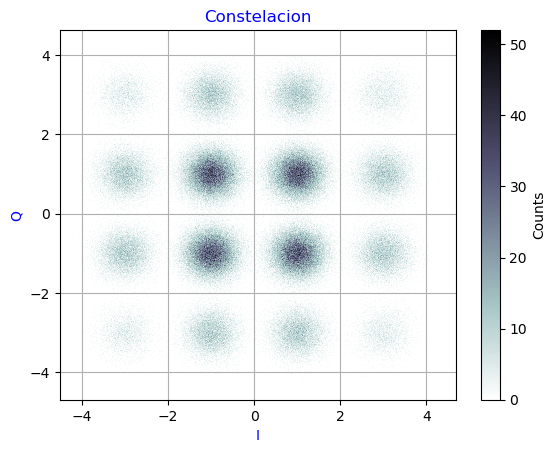
\includegraphics[width=\textwidth]{Graficos/Constellation_025.png}
%     \end{figure}
%     \end{column}
% \end{columns}
% \end{frame}


% \begin{frame}
%   \frametitle{\textbf{Resultados obtenidos}}
%\framesubtitle{\secname : \subsecname}
%   Sin realizar codificación:
% \begin{columns}
%     \begin{column}{0.48\paperwidth}  
%     \begin{figure}
%         \centering
%         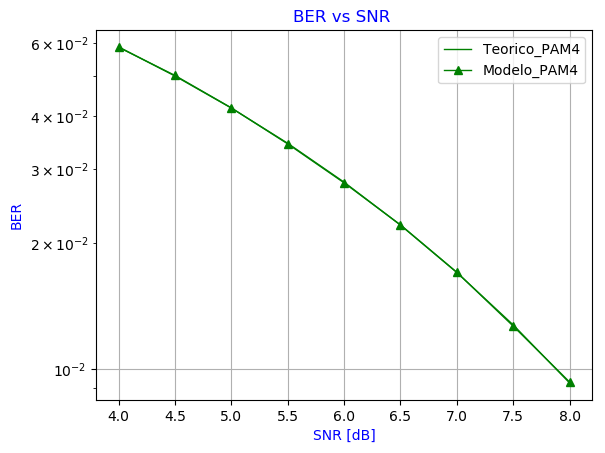
\includegraphics[width=\textwidth]{Graficos/BER_vs_SNR_1.png}%
%     \end{figure}
%     \end{column}

%     \begin{column}{0.48\paperwidth}
%     \begin{figure}
%         \centering
%         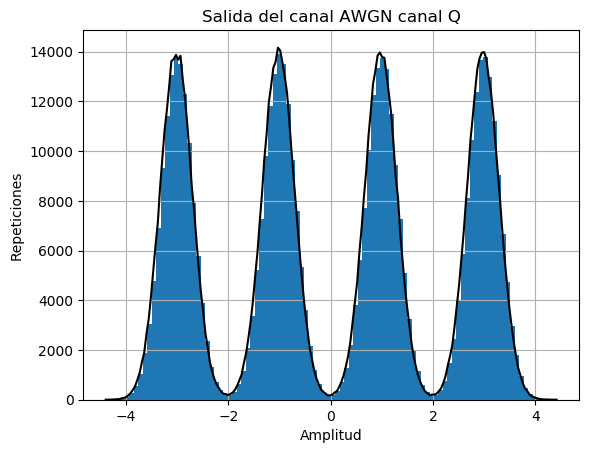
\includegraphics[width=\textwidth]{Graficos/AWGN_symbols.png}
%     \end{figure}
%     \end{column}
% \end{columns}
% \end{frame}

\begin{frame}
  \frametitle{\textbf{Penalidad por redundancia}}
\framesubtitle{\secname : \subsecname}
   \begin{block}{}
    \begin{itemize}
    \item De los 16 bits transmitidos solo 12 son de información.
    \item Se produce un desplazamiento en la curva dado por la ecuación $ 10.log(16/12)\approx1,25\, dB$
    \item Esto se conoce como `Overhead' (OH).
    \end{itemize}
    \end{block}
       \vspace{-0.3cm}
    \begin{figure}
      \centering
      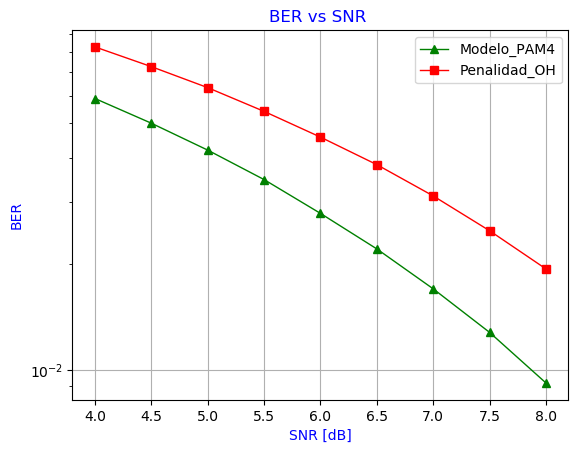
\includegraphics[width=0.50\paperwidth]{Graficos/BER_vs_SNR_2.png}%
    \end{figure}
\end{frame}

\begin{frame}
  \frametitle{\textbf{Ganancia por potencia}}
\framesubtitle{\secname : \subsecname}
   \begin{block}{}
    \begin{itemize}
    \item La potencia transmitida está dada por:
        \begin{equation*}
            P_{tx} = P_{(s = 1)}  (1)^{2} + P_{(s = 3)}  (3)^{2}
        \end{equation*}
    \item Para $ P_{(s = 3)}=0.25$ se obtiene una reducción de potencia del 40\% respecto a $ P_{(s = 3)}=0.50$.
    % \item SNR constante. 
    \end{itemize}
    \end{block}
     \vspace{-0.3cm}

   \begin{figure}
  \centering
  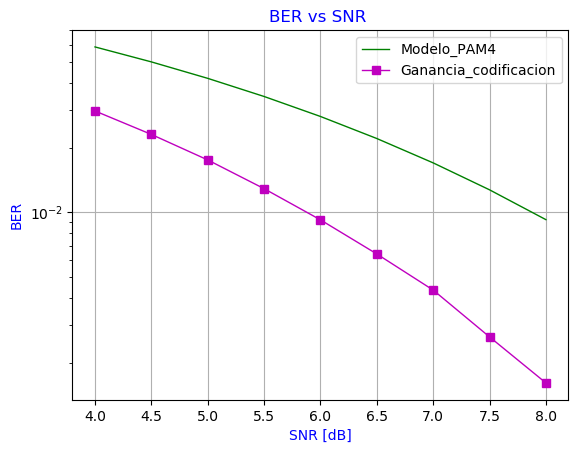
\includegraphics[width=0.45\paperwidth]{Graficos/BER_vs_SNR_3.png}%
\end{figure}
\end{frame}


\begin{frame}
  \frametitle{\textbf{Multiplicación de errores}}
\framesubtitle{\secname : \subsecname}
      \begin{block}{}

   \begin{itemize}\small
    \item Un error de un bit transmitido puede verse reflejado en hasta 4 bits a la salida
 del decodificador.
 \item Considerando este efecto, el sistema presenta un mejor desempeño que una modulación PAM-4 para una SNR mayor a 7dB.
 \end{itemize}
 \end{block}
     \vspace{-0.3cm}

\begin{columns}
    \begin{column}{0.65\paperwidth}
    \begin{figure}
        \centering
        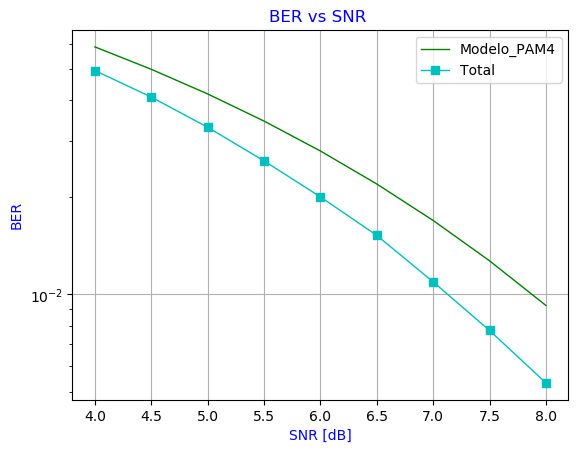
\includegraphics[width=0.45\textwidth]{Graficos/BER_vs_SNR_4.png}%
        \label{fig:my_label}
    \end{figure}

    \end{column}
    \begin{column}{0.65\paperwidth}  
    
    \begin{figure}
        \centering
        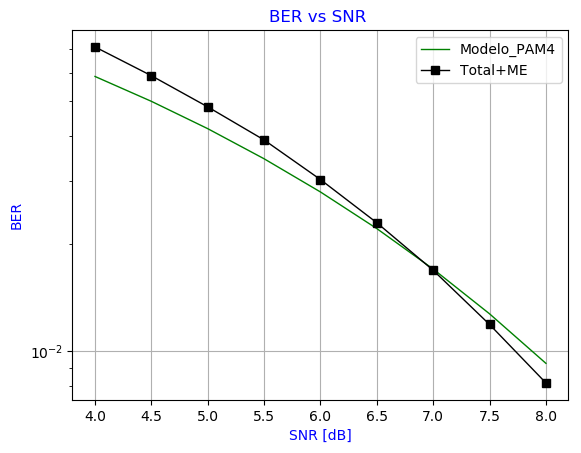
\includegraphics[width=0.45\textwidth]{Graficos/BER_vs_SNR_5.png}
        \label{fig:my_label}
    \end{figure}
    
    \end{column}
\end{columns}
\end{frame}

\begin{frame}
  \frametitle{\textbf{Modelo final}}
\framesubtitle{\secname : \subsecname}
      \begin{block}{}
        % \begin{itemize}
        %     \item Disminución de potencia
        %     \item Penalidad por redundancia 
        %  \end{itemize}
        \begin{itemize}
            \item Comparación con QAM8. 
            \item Secuencia de entrada de 100 bits.
            \item Probabilidad de $P_{(s=3)} = 0.12$.
     \end{itemize}  
     \end{block}
    \vspace{-0.3cm}

\begin{columns}
    % \begin{column}{0.48\paperwidth}
    % \begin{figure}
    %     \centering
    %     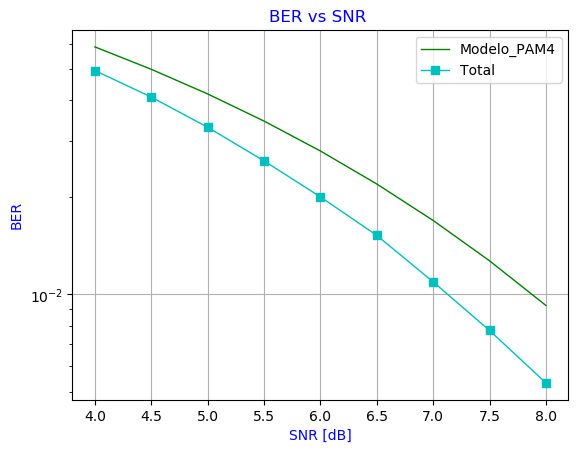
\includegraphics[width=\textwidth]{Graficos/BER_vs_SNR_4.png}%
    %     \label{fig:my_label}
    % \end{figure}
    % \end{column}
    
    \begin{column}{0.48\paperwidth}  
    \begin{figure}
        \centering
        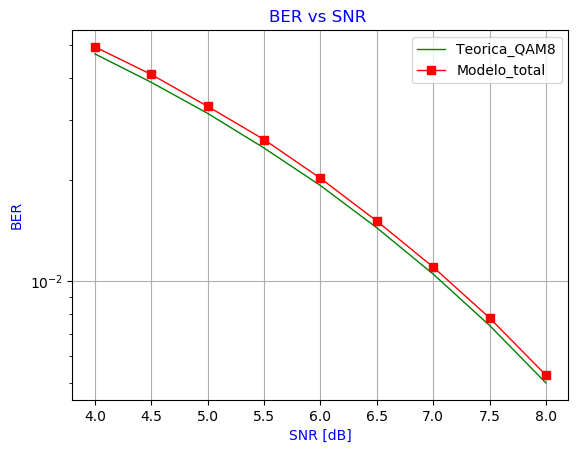
\includegraphics[width=\textwidth]{Graficos/BER_vs_SNR_6.png}
        \label{fig:my_label}
    \end{figure}
    \end{column}
    
    \begin{column}{0.48\paperwidth} 
        \begin{figure}
          \centering
          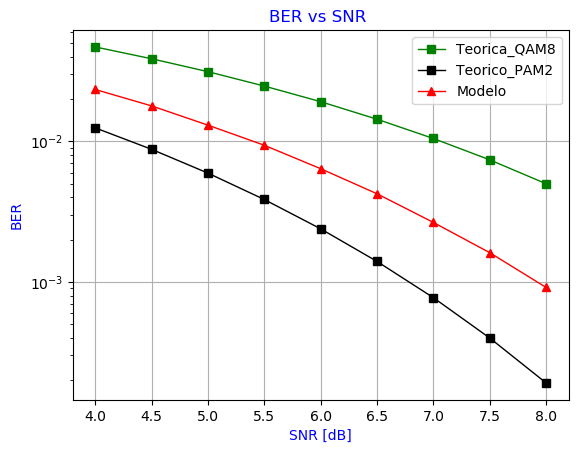
\includegraphics[width=\textwidth]{Graficos/BER_vs_SNR_8.png}%
        \end{figure}
        \end{column}
    \end{columns}

\end{frame}

% \begin{frame}
%   \frametitle{\textbf{Modelo final}}
%      \framesubtitle{\secname : \subsecname}
%   \begin{block}{\centering \textbf{Si se considera:}}
  
%     \end{block}
%     \vspace{-0.3cm}
 
% \end{frame}


\begin{frame}
  \frametitle{\textbf{Umbral de decisión}}
\framesubtitle{\secname : \subsecname}
      \begin{block}{\centering \textbf{Umbral de decisión}}
  \begin{itemize}
    \item Mejora en el desempeño.
    \item La diferencia se reduce a medida que la SNR aumenta.  
 \end{itemize}
    \end{block}
\vspace{-0.3cm}
\begin{columns}
    \begin{column}{0.48\paperwidth}
     \begin{figure}
      \centering
      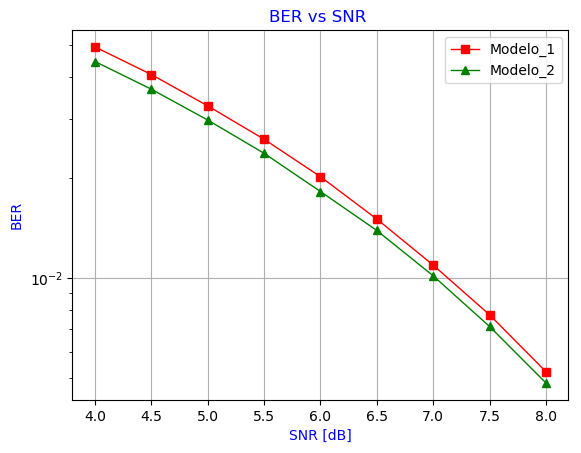
\includegraphics[width=\textwidth]{Graficos/BER_vs_SNR_9.png}%
    \end{figure}
    
    \end{column}
    \begin{column}{0.48\paperwidth}  
    \begin{figure}
        \centering
         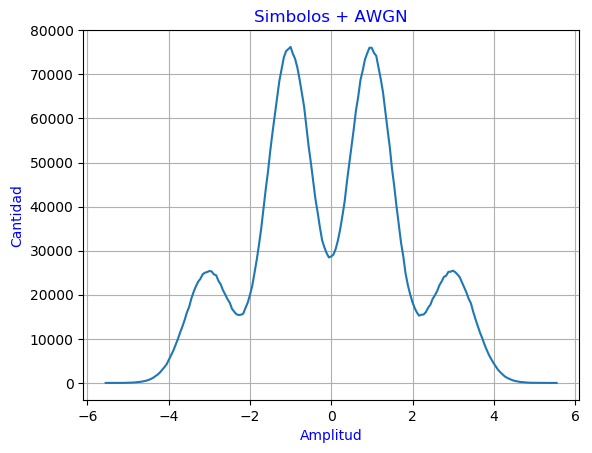
\includegraphics[width=\textwidth]{Graficos/Slicer_025.png}
    \end{figure}
   
    \end{column}
\end{columns}
\end{frame}


\begin{frame}
  \frametitle{\textbf{Umbral de decisión}}
\framesubtitle{\secname : \subsecname}
     \begin{block}{\centering \textbf{Umbral de decisión}}
     \begin{itemize}
        \item Está dado por: 
             \begin{equation*}
            P_{(s=1)}* exp{(\frac{-(\tau-1)}{2{\sigma}^{2}})} =  P_{(s=3)}* exp{(\frac{-(\tau-3)}{2{\sigma}^{2}})}
            \end{equation*}
    \item Donde:
    \begin{description}\footnotesize
    \item [$\tau:$] Umbral de decisión.
    \item [$\sigma^2:$] Varianza del ruido.
    \end{description}
    \item  Para $P_{(s=1)}=0.75$ :
        \begin{equation*}
            \tau = 2 + 0.55  *{\sigma}^{2}
        \end{equation*}
    \end{itemize}
    \end{block}
\end{frame}